%\GB{I suggest: ``Attacks against Migration'' as a title}
\label{sec:attacker-model}
The migration of a VT creates nodes, virtual links, and instantiates the links between nodes.
Thus, based on  the migration primitives we introduced in Section~\ref{sec:migration} and the axioms we have presented in Section~\ref{sec:prop-conf}, 
%\GB{I am wondering if it s not better to move SNARK explanation closer to the experiments and having migration and security properties close to each other}\FC{To be debated}\GB{what's the more with the new structure suggested by moving Migration section after RW section}, we can illustrate the possibilities an attacker has to affect a virtual topology.
we will describe the different components of a threat using the following syntax
%\GB{terms?}
%\FC{The syntax is the combination of terms}
: Attacker - Action - Target.

\begin{figure}[t!]
\centering
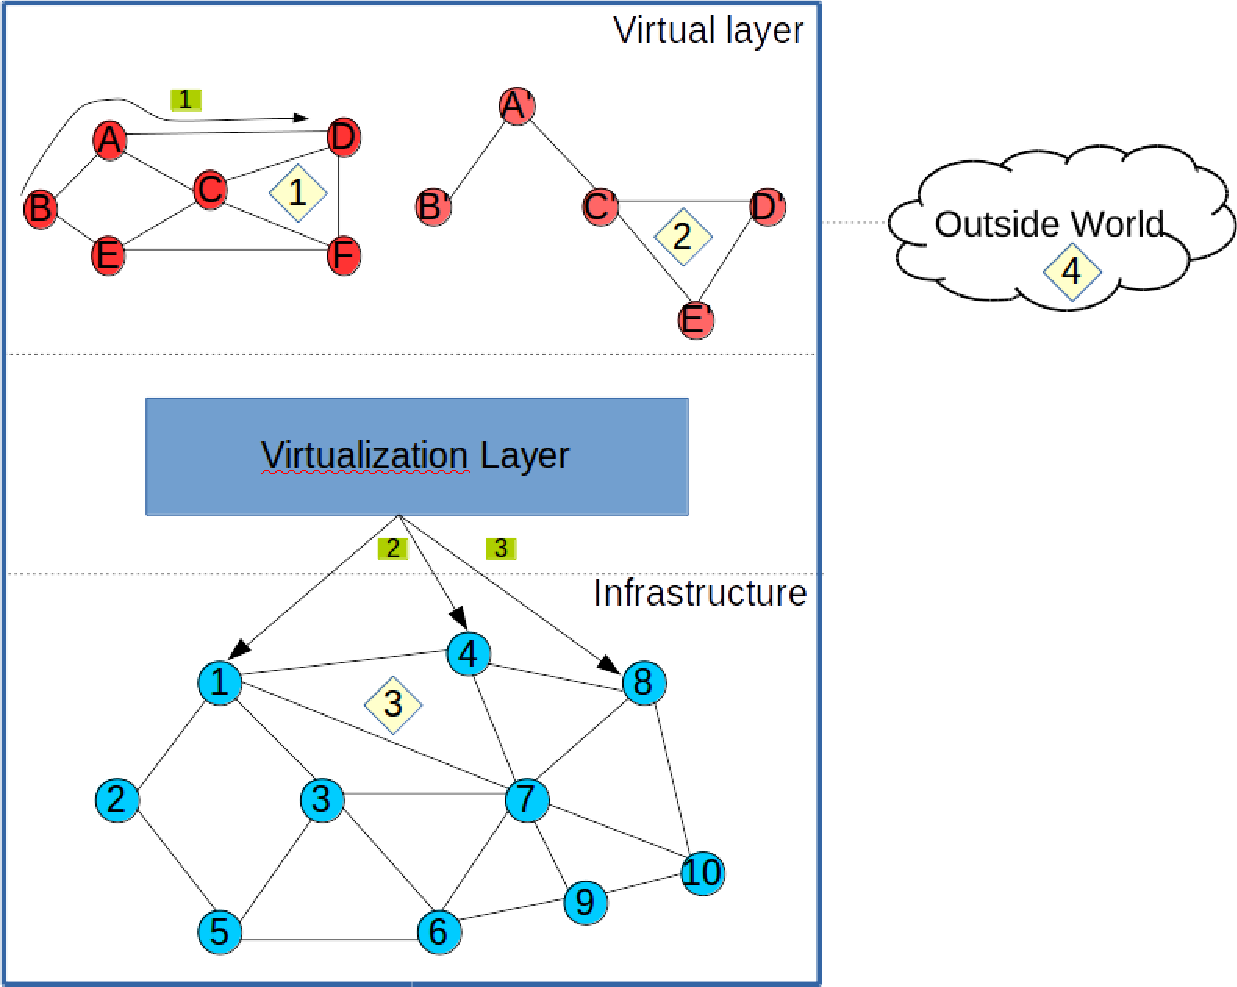
\includegraphics[scale=0.85]{figures/virtualization-attack-surface}
\caption{Attack surface of the SDN environment.\label{fig:attack-surface}}
\end{figure}

\subsubsection{Attacker}
We consider the different locations from where an attacker could attack the migration of the VT. 
Figure~\ref{fig:attack-surface} places four different attackers (identified by diamonds): 
\begin{inparaenum}[(1)] 
\item the insider, 
\item the collocated user, 
\item the provider and
\item the outsider.
\end{inparaenum}
The insider is an attacker located inside the VT that is going to be migrated.
It can be a malicious user able to control a virtual node and deploy incorrect flow rules.
"The collocated user is another user of the virtualization platform.
He can use his own topology on the physical infrastructure.
The provider is the owner of the physical infrastructure.
He has access to the SDN switches embedding the virtual topologies.
The outsider is a malicious user outside the SDN environment.
He has limited access to both the VTs and the physical infrastructure.

\subsubsection{Action}
There are 4 major actions that can be performed by an attacker to affect the VTs and their environment.
The first two are related to the infrastructure and the others are related to the data carried across the network.
\begin{itemize}
\item Unauthorized access to a network element.
\item Disruption of service on a network element.
\item Information disclosure without authorization.
\item Information modification or destruction without authorization.
\end{itemize}

\subsubsection{Target}
We can consider two types of targets: nodes or data.
The nodes are either the physical switches in the infrastructure or the virtual nodes of a VT.
There are three types of data inside a VT and its infrastructure.
The user data carried by the virtual elements, the management data and the configuration data carried by the infrastructure. 
We place the different data flows on Figure~\ref{fig:attack-surface}.
\begin{enumerate}
\item User data
\item Management data
\item Configuration data
\end{enumerate}
%\GB{how can you make the difference between the management and configuration data? it seems to me that both data are born by the SBI protocol. However, should we consider the flow within the substrate network?}
%\FC{Both 2 and 3 are generated by the SBI but are of different nature. One are flow rules, the other are hello packets and similar. What would you use in the substrate network ?}

The user data is the traffic generated by the user and going through the VT.
The management data is made of the different packets exchanged between the virtualization layer and the physical infrastructure to operate properly (capacities, established links, etc.).
The configuration data are the different flow rules deployed on the physical switches when instantiating a VT%\GB{configuration should be considered as not a flow but immobile data stored at the switches}\FC{These are flow rules. As described earlier, the virtual topology is a collection of flow rules. Therefore, the configuration data (i.e. data describing the VT) is composed of flow rules}.

\subsubsection{Attacks}
%\GB{What about just ``Attacks'' as a title?}
\label{sec:attacks}
%\GB{please in this section and the following, specify which attack is directed against which algorithm}
In the previous subsections, we have defined the different attackers, as well as the malevolent actions and possible targets in the virtualization infrastructure. 
Table~\ref{tab:attack-model} summarizes these information.
We will now combine these elements to define several attacks targeting the migration process or the user's data.
In this paper, we chose to focus on the security aspects of the confidentiality.
Thus, we are more interested in the unauthorized access and information disclosure of the attack model.
As we also consider a stable initial environment, an outsider attacker is too limited to attack the infrastructure and is therefore of no interest in this paper.
Finally, the different data present in the threat model are similar enough in essence.
Attacking one or another makes no difference in terms of formal modeling.
We propose two different attacks, one focusing on the disclosure of confidential traffic carried by a VT, and the other will be an on-site attack on a physical node.
%\GB{please specify which migration algorithms are attacked here, and in the next section}

%\GB{in general, you could sum up in a table what attacker can do what against what. I am surprised that you only have two scenarios. Usually attacker classes tend to be ordered sets. But it is not always the case}
%\FC{I believe one attack scenario per migration algorithm is enough. However I agree with the table, will work on it today. I don't understand what you mean by ordered sets.}
%\GB{usually, you describe different attackers that share abilities, from the least potent to the most potent. Usually the least potent has ability to perform action A, then the second least potent can do actions A and B, then another can do actions A, C and D, and the most potent can do A, B, C and D. If you are presenting only a couple of scenarios, you may actually list all possible scenarios, \ie triplets (Attacker, Action, Target) and explicitly state that you will only demonstrate two of them, motivating why you choose these}

\begin{table}[h]
\centering
\begin{tabular}{|l|l|l|}
\hline
\textbf{Attacker}   & \textbf{Action}    & \textbf{Target}             \\ \hline
Insider    & Unauthorized access                  & Nodes              \\ \hline
Collocated & Disruption of service                & User data          \\ \hline
Provider   & Information disclosure               & Management data    \\ \hline
Outsider   & Information modification/destruction & Configuration data \\ \hline
\end{tabular}
\caption{Elements of the attack model}
\label{tab:attack-model}
\end{table}

\paragraph{Information disclosure} In this scenario, the attacker is a collocated user that is gaining access to another user's traffic. 
We consider a number of assumptions. 
First, the attacker is aware that a migration is ongoing. 
He can force it by attacking the victim's topology or the infrastructure beneath it.
For instance, he can exhaust the infrastructure's capacities by asking for more and more network resources, or by congesting the network links.
%\GB{the remainder of the sentence is long and confusing. Tobe rewritten} or by requesting migrations on the infrastructure set currently occupied by the victim so the virtualization layer may be forced to relocate the victim's topology somewhere else, thus giving an opportunity to the attacker.
%\GB{what about requesting more resources, forcing a migration of nodes, incl. both VMs and switches?}. 
%\FC{Do you mean we should be more detailed about the attack ?}
%\GB{Yes!}
Second, he must be aware of where the new embedding will deploy the topology. 
Deploying probes in the network or attacking on a large scale the infrastructure could lead the virtualization layer to a particular deployment. 
Finally, the attacker must be able to perform an attack that will disclose information.
In~\cite{Costa2015,Sphinx-Dhawan2015}, are described a number of methods to achieve this disclosure. 
%\GB{Is the following two sentences examples from the cited paper?}\FC{Yes} One is to insert flow rules with particular parameters that will extract the confidential data. 
The other is to create a fake link inside the infrastructure so the virtualization layer will deploy the virtual topology on it. 

\paragraph{Node exploitation} We now consider a malicious user that is going to compromise several virtual topologies by attacking a single physical node. 
The attacker is located on the provider side, however, he does not have access to the whole infrastructure.
Typically, it could be an employee of the provider having only access to some physical equipments.
The attacker has physical access to a single switch and is able to alter the flow rules installed on it.
Retrieving the different flow rules installed on the switch gives access to a fragment of all the virtual topologies deployed on it.
The predicates affected by this attack are: $accesses, node\_is\_authorized, data\_confidentiality$.
Therefore, it becomes possible to begin a partial mapping of the different users in the infrastructure, thus disclosing configuration data.
%\GB{would it violate any of the confidentiality axioms you have defined?}.
%\FC{Yes because of the unauthorized access to a confidential data}
%\GB{Ok, that what I thought. But just in case, being more explicite about it will not hurt. It good to say that you expect the malevolent action to trigger a particular predicate.}
%Altering the flow rules in a node allows for Man-In-The-Middle attacks by redirecting data toward another node that will log incoming traffic before sending it back to its legitimate destination.